% When using TeXShop on the Mac, let it know the root document. The following must be one of the first 20 lines.
% !TEX root = ../design.tex

\chapter[Singular Value Decomposition]{Singular Value Decomposition}

\begin{moduleinfo}
\item[Author] \href{mailto:riyer@gopivotal.com}{Rahul Iyer}
\item[History]
    \begin{modulehistory}
        \item[v0.1] Initial version
    \end{modulehistory}
\end{moduleinfo}

\newcommand{\vectornorm}[1]{\left|\left|#1\right|\right|}
\def\Rset{\mathbb{R}}
% Abstract. What is the problem we want to solve?
In linear algebra, the singular value decomposition (SVD) is a factorization of
a real or complex matrix, with many useful applications in signal processing and
statistics.

Let $A$ be an $m \times n$ matrix, where $m \ge n$. Then $A$ can be decomposed as follows:
\begin{gather*}
    A = U \Sigma V^T,
\end{gather*}
where $U$ is a $m \times n$ orthonormal matrix, $\Sigma$ is a $n\times n$
diagonal matrix, and $V$ is an $n\times n$ orthonormal matrix. The diagonal
elements of $\Sigma$ are called the \emph{singular values}.

It is possible to formulate the problem of computing the singular triplets
($\sigma_i, u_i, v_i$) of $A$ as an eigenvalue problem involving a Hermitian
matrix related to $A$. There are two possible ways of achieving this:

\begin{figure}[tb]
    \begin{center}
        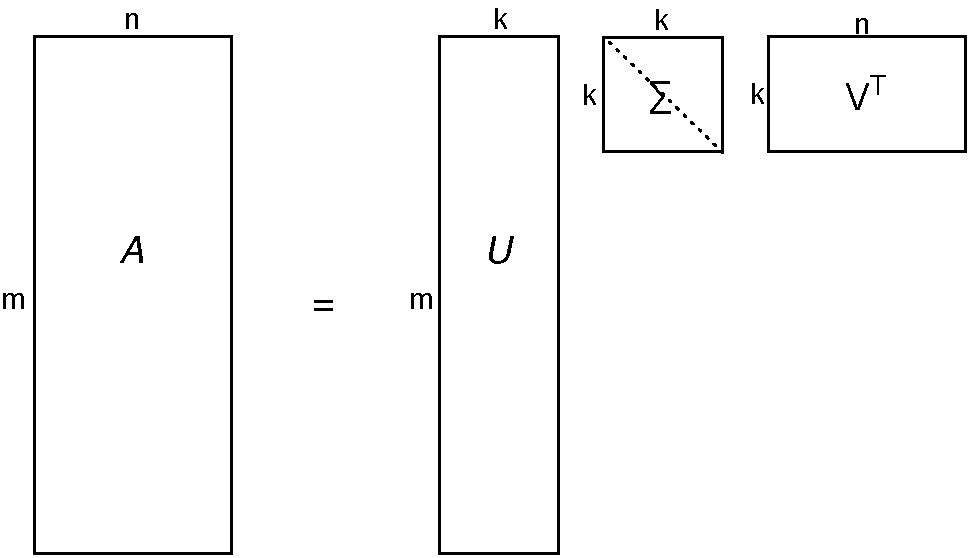
\includegraphics[width=\textwidth]{figures/svd_figure}
    \end{center}
    \caption{Singular Value Decomposition}
    \label{fig:svd}
\end{figure}

\begin{enumerate}
    \item With the cross product matrix, $A^TA$ and $AA^T$
    \item With the cyclic matrix $H(A) =
        \begin{bmatrix}
            0   & A\\
            A^* & 0
        \end{bmatrix}$
\end{enumerate}

The singular values are the nonnegative square roots of the eigenvalues of the
cross product matrix. This approach may imply a severe loss of accuracy in the
smallest singular values. The cyclic matrix approach is an alternative that
avoids this problem, but at the expense of significantly increasing the cost of
the computation.

Computing the cross product matrix explicitly is not recommended, especially in
the case of sparse A. Bidiagonalization was proposed by Golub and
Kahan~\cite{golub1965} as a way of tridiagonalizing the cross product matrix
without forming it explicitly.

Consider the following decomposition
\begin{gather*}
    A = P B Q^T,
\end{gather*}

where P and Q are unitary matrices and B is an $m\times n$ upper bidiagonal
matrix. Then the tridiagonal matrix $BB^T$ is unitarily similar to $AA^T$.
Additionally, specific methods exist that compute the singular values of $B$
without forming $BB^T$. Therefore, after computing the SVD of B,
\begin{gather*}
    B = X \Sigma Y^T,
\end{gather*}
it only remains to compute the SVD of the original matrix with $U = PX$ and $V = QY$.

\section{Lanczos Bidiagonalization} % (fold)
\label{sec:lanczos_bidiagonalization}

The Lanczos algorithm is an iterative algorithm devised by Cornelius Lanczos
that is an adaptation of power methods to find eigenvalues and eigenvectors of a
square matrix or the singular value decomposition of a rectangular matrix. It is
particularly useful for finding decompositions of very large sparse matrices.

For a rectangular matrix $A$, the Lanczos bidiagonalization method computes a
sequence of Lanczos vectors $p_j \in \mathbb{R}^m$ and $q_j \in \mathbb{R}^n$
and scalars $\alpha_j$ and $\beta_j$ for $j = 1, 2, \ldots, k$ as follows:

\begin{algorithm}[Lanczos Bidiagonalization Algorithm]
 % \label{alg:lanczos-bidiagonalization}
\begin{algorithmic}[1]
     \State Choose a unit-norm vector $q_1$ and let $\beta_0 = 0$ and $p_0 = 0$
     \For{$j = 1, 2, \ldots, k$}
        \State $p_j \set Aq_j - \beta_{j-1} p_{j-1}$
        \State $\alpha_j \set \vectornorm{p_j}_2$
        \State $p_j \set p_j/\alpha_j$
        \State $q_{j+1} \set A^Tp_j - \alpha_j q_j$
        \State $\beta_j \set \vectornorm{q_{j+1}}_2$
        \State $q_{j+1} \set q_{j+1}/\beta_j$
    \EndFor
\end{algorithmic}
\end{algorithm}


After $k$ steps, we can generate the bidiagonal matrix $B_k$ as follows,
\[
\begin{bmatrix}
    \alpha_1    & \beta_1   &           &           &               & \\
                & \alpha_2  & \beta_2   &           &               & \\
                &           & \alpha_3  & \beta_3   &               & \\
                &           &           & \ddots    & \ddots        & \\
                &           &           &           & \alpha_{k-1}  & \beta_{k-1} \\
                &           &           &           &               & \alpha_k
\end{bmatrix}
\]
In exact arithmetic the Lanczos vectors are orthonormal such that,
\begin{gather*}
    P_{k+1} = (p_1, p_2, \dotsc, p_{k+1}) \in \mathbb{R}^{m \times (k+1)},
        P_{k+1}^T P_{k+1} = I_{k+1} \\
    Q_{k+1} = (q_1, q_2, \dotsc, q_{k+1}) \in \mathbb{R}^{n \times  (k+1)},
        Q_{k+1}^T Q_{k+1} = I_{k+1}.
\end{gather*}

\begin{figure}[tb]
    \centering
        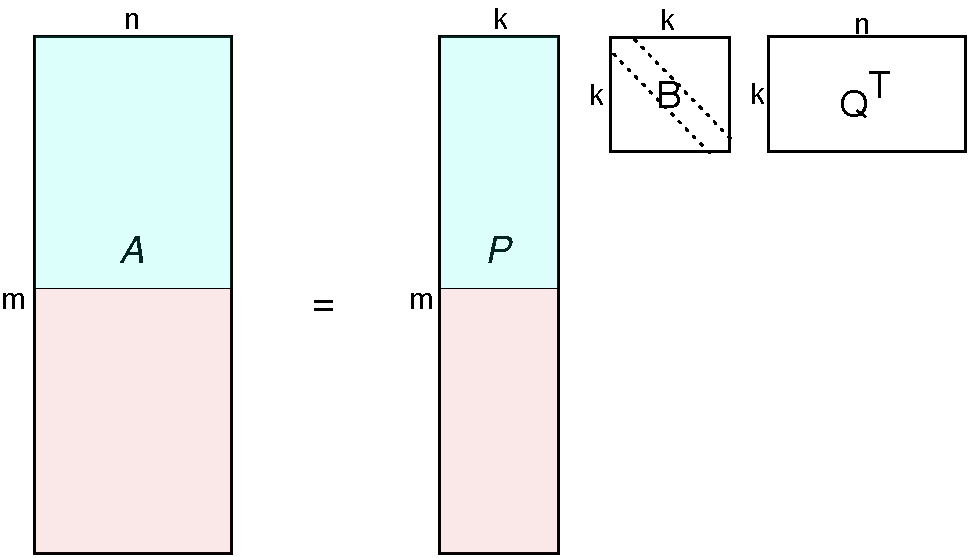
\includegraphics[width=\textwidth]{figures/lanczos_bidiag_segment}
    \caption{Lanczos bidiagonalization of $A$}
    \label{fig:lanczos}
\end{figure}
After $k$ Lanczos steps, the Ritz values $\tilde{\sigma_i}$ (approximate singular
values of A) are equal to the computed singular values of $B_k$, and the
Ritz vectors are
\begin{gather*}
    \tilde{u_i} = P_k x_i,  \qquad  \tilde{v_i} = Q_k y_i
\end{gather*}
% subsubsection lanczos_bidiagonalization (end)

\section{Dealing with Loss of Orthogonality} % (fold)
\label{sec:dealing_with_loss_of_orthogonality}

After a sufficient number of steps the Lanczos vectors start to lose their
mutual orthogonality, and this happens together with the appearance in the
spectrum of $B_j$ of repeated and spurious Ritz values. The simplest cure for
this loss of orthogonality is full orthogonalization. In Lanczos
bidiagonalization, two sets of Lanczos vectors are computed, so full
orthogonalization amounts to orthogonalizing vector $p_j$ explicitly with
respect to all the previously computed left Lanczos vectors, and orthogonalizing
vector $q_{j+1}$ explicitly with respect to all the previously computed right
Lanczos vectors.

\begin{algorithm}[Lanczos Bidiagonalization with Partial Reorthogonalization]
% \label{alg:one-sided_lanczos}
\begin{algorithmic}[1]
     \State Choose a unit-norm vector $q_1$ and let $\beta_0 = 0$ and $p_0 = 0$
     \For{$j = 1, 2, \ldots, k$}
        \State $p_j \set Aq_j - \beta_{j-1} p_{j-1}$
        \State $\alpha_j \set \vectornorm{p_j}_2$
        \State $p_j \set p_j/\alpha_j$
        \State $q_{j+1} \set A^Tp_j - \alpha_j q_j$
        \State Orthogonalize $q_{j+1}$ with respect to $Q_j$
        \State $\beta_j \set \vectornorm{q_{j+1}}_2$
        \State $q_{j+1} \set q_{j+1}/\beta_j$
    \EndFor
\end{algorithmic}
\end{algorithm}

There is a variation of this orthogonalization that maintains the effectiveness
of full reorthogonalization but with a considerably reduced cost. This technique
was proposed by Simon and Zha~\cite{simon2000}. The idea comes from the observation that,
in the Lanczos bidiagonalization procedure without reorthogonalization, the
level of orthogonality of left and right Lanczos vectors go hand in hand. This
observation led to Simon and Zha to propose what they called the one-sided version
shown in Algorithm~2. %\ref{alg:one-sided_lanczos}.
% section dealing_with_loss_of_orthogonality (end)

\section{Enhancements for Distributed Efficiency} % (fold)
\label{sec:parallelizing}

\begin{algorithm}[Distributed version of Lanczos BPRO]% \label{alg:one-sided_lanczos}
\begin{algorithmic}[1]
     \State Choose a unit-norm vector $q_1$ and let $\beta_0 = 0$ and $p_0 = 0$
     \For{$j = 1, 2, \ldots, k$}
        \Statex {\footnotesize Transition step}
        \State $p_j \set Aq_j - \beta_{j-1} p_{j-1}$
        \State $\alpha_j \set \vectornorm{p_j}_2^2$   \Comment Delayed normalization
        \State $q_{j+1} \set A^Tp_j - \alpha_j q_j$
        \Statex {\footnotesize Merge step}
        \State Concatenate $p_j$ across parallel segments
        \State Sum $q_{j+1}$ across parallel segments
        \Statex {\footnotesize Final Step}
        \State $\alpha_j \set \sqrt{\alpha_j}$
        \State $p_j \set p_j/\alpha_j$
        \State $q_j \set q_j/\alpha_j$
        \State Orthogonalize $q_{j+1}$ with respect to $Q_j$
        \State $\beta_j \set \vectornorm{q_{j+1}}_2$
        \State $q_{j+1} \set q_{j+1}/\beta_j$
    \EndFor
\end{algorithmic}
\end{algorithm}

% section parallelizing (end)
